% Czym jest replikacja, problemy, modele spójności: dano- i klientocentryczne
\chapter{Problematyka replikacji danych} \label{chapter:replication}

Niniejszy rozdział poświęcony jest omówieniu problematyki replikacji danych. Zawiera on przedstawienie modelu systemu rozproszonego, którego dotyczyć będą rozważania w dalszej części pracy, wyjaśnienie pojęcia replikacji, powody, dla których jest to powszechnie stosowana technika zarówno w istniejących, jak i nowo tworzonych systemach informatycznych oraz trudności związanych z utrzymaniem spójności zwielokrotnianych danych. Opisane zostaną także istniejące modele spójności, gwarantujące zachowanie pewnych reguł w systemie podczas przeprowadzania aktualizacji replikowanych danych, wraz z ich podziałem na modele dano- i klientocentryczne.

\section{Model systemu rozproszonego} \label{section:system_model}

System rozproszony składa się z dwóch elementów:
% [MB] Głowy nie dam sobie uciąć, ale kursywy powinniśmy raczej używać raczej jeśli mamy zwrot obcojęzyczny, który używamy jako objaśnienie terminu polskojęzycznego
% [BK] Ok, wyrzucam kursywy

\begin{itemize}
    \item środowiska przetwarzania rozproszonego,
    \item zbioru procesów rozproszonych
\end{itemize}

Środowisko przetwarzania rozproszonego jest zbiorem $ \mathcal{N} $ autonomicznych jednostek przetwarzających $ \textbf{N}_i $ (nazywanych węzłami), zintegrowanych siecią komunikacyjną. Każdy z węzłów jest wyposażony w procesor, lokalną pamięć oraz interfejs komunikacyjny. Nie występuje tutaj pamięć współdzielona przez węzły, dlatego komunikacja pomiędzy nimi odbywa się wyłącznie poprzez wymianę wiadomości (komunikatów).

Drugim elementem jest zbiór procesów rozproszonych $ \mathcal{P} $, składający się z procesów sekwencyjnych $ \emph{P}_i \in \mathcal{P} $, realizujących współbieżnie i w skoordynowany sposób wspólne cele przetwarzania rozproszonego.

Wyróżniamy systemy rozproszone synchroniczne i asynchroniczne. Niniejsza praca zakłada istnienie systemu asynchronicznego, co oznacza, że poszczególne węzły wykonują operacje z różnymi prędkościami w takt niezależnych zegarów, a czas transmisji wiadomości jest skończony lecz nieznany.

Należy zaznaczyć również, że rozpatrujemy model systemu w topologii kliki, co oznacza, że każdy
węzeł systemu posiada bezpośrednie połączenie z każdym innym węzłem. W niniejszej pracy dodatkowo
zakładamy dostępność niezawodnych kanałów typu FIFO (ang.\ \textit{first in, first out}), z powodów opisanych w rozdziale dotyczącym implementacji proponowanego systemu składowania danych.

\section{Pojęcie replikacji}

% [MB] to samo co powyżej

Replikacja polega na utrzymywaniu wielu kopii tych samych danych lub obiektów na wielu, niezależnych węzłach. Technikę tę stosuje się powszechnie w systemach rozproszonych, przy czym główną motywacją do jej użycia jest potencjalne zwiększenie efektywności oraz niezawodności przetwarzania. Z założenia modyfikacje replikowanych danych mają miejsce na pojedynczych kopiach, natomiast użytkownicy mogą odwoływać się do każdej z istniejących kopii. Powoduje to powstawanie problemów związanych ze spójnością przechowywanych danych, będących potencjalnymi źródłami poważnych błędów w tworzonych aplikacjach.

\section{Modele spójności}

% [MB] jw. "modelu spójności", "protokół spójności". Ewentualnie można pogrubić te fragmenty, ale to pasuje chyba bardziej do artykułów popularnonaukowych

Pod pojęciem modelu spójności rozumiemy gwarancje dotyczące spójności replik w odniesieniu do uporządkowania operacji realizowanych przez system. Aplikacje, dla których gwarancje te są wystarczające będą działały poprawnie pomimo istnienia zwielokrotniania, opóźnień i czasowych niespójności danych.

W celu nadania praktycznego znaczenia pojęciu modelu spójności należy skonstruować odpowiadający mu protokół spójności, który zapewni w systemie rozproszonym spełnienie gwarancji zawartych w modelu spójności. Protokół spójności określa kiedy i w jaki sposób należy ingerować w przetwarzanie, aby zachować własności zdefiniowane na poziomie modelu spójności.

W ogólności, modele spójności można podzielić na dwie grupy:
\begin{itemize}
    \item modele nastawione na dane (danocentryczne),
    \item modele nastawione na klienta (klientocentryczne)
\end{itemize}
W następnych punktach omówione zostaną obie grupy wraz z przykładowymi modelami należącymi do każdej z nich. Zanim jednak to nastąpi konieczne jest jasne i ścisłe zdefiniowanie modelu systemu rozproszonego, którego dotyczyć będą definicje modeli spójności.

\subsection{Przyjęte założenia i oznaczenia}

Niniejsza praca zakłada istnienie systemu rozproszonego, zgodnie z założeniami opisanymi w punkcie \ref{section:system_model}, jednak dodatkowo zakłada istnienie skończonego zbioru współdzielonych zmiennych $ X = \{x_1, x_2, ...\} $, a każdy z procesów $ \emph{P}_i \in \mathcal{P} $ posiada własną replikę całego zbioru $ X $ oraz może realizować na zmiennej $ x_i \in X $ operacje:
\begin{itemize}
    \item zapisu wartości $ v $, co oznaczać będziemy $ w_i(x)v $,
    \item odczytu wartości $ v $, co oznaczać będziemy $ r_i(x)v $
\end{itemize}
Realizacja każdej z tych operacji przebiega w dwóch fazach:
\begin{itemize}
    \item żądanie operacji (ang.\ \textit{operation issue})
    \item wykonanie operacji (ang.\ \textit{operation execution})
\end{itemize}
Osobne oznaczenia wprowadzono także dla rozróżnienia zbiorów operacji wykonanych w systemie:
\begin{itemize}
    \item $ O $ to zbiór wszystkich operacji w systemie
    \item $ O_i $ to zbiór operacji procesu $ P_i $
    \item $ OW $ to zbiór wszystkich operacji zapisu w systemie
    \item $ O|_x $ to zbiór wszystkich operacji dotyczących zmiennej $ x $
\end{itemize}
Różne porządki operacji wykonywanych w systemie oznaczane są następująco:
\begin{itemize}
    \item $ \rightarrow_i $ to lokalny porządek wykonania operacji przez proces $ P_i $
    \item $ \rightarrow $ to porządek przyczynowy
    \item $ \mapsto_i $ to uszeregowanie operacji postrzegane przez proces $ P_i $
\end{itemize}

\subsubsection{Porządek przyczynowy} \label{section:causal_order}

W tym miejscu należy zdefiniować pojęcie \textit{porządku przyczynowego}, ponieważ odwołuje się do niego model spójności przyczynowej, czyli jeden z modeli spójności nastawionych na dane. Jest on definiowany za pomocą poniższych trzech warunków:
\begin{enumerate}
    \item{\makebox[2cm][l]{$ \forall_{o_1, o_2 \in O_i} $} 
        $ (o_1 \rightarrow_i o_2 \Rightarrow o_1 \rightarrow o_2) $ }
    \item{\makebox[2cm][l]{$ \forall_{x \in X} $}
        $ w(x)v \rightarrow r(x)v $ }
    \item{\makebox[2cm][l]{$ \forall_{o_1, o_2, o \in H} $}
        $[(o_1 \rightarrow o \wedge o \rightarrow o_2) \Rightarrow o_1 \rightarrow o_2] $ }
\end{enumerate}
Warunek pierwszy mówi o tym, że lokalne uporządkowanie operacji wykonywanych przez poszczególne węzły jest zachowywane przez porządek przyczynowy. Punkt drugi oznacza, że jeśli w systemie nastąpił odczyt wartości $ v $ ze zmiennej $ x $, to operacja zapisu tej wartości do zmiennej $ x $ musi przyczynowo poprzedzać operację jej odczytu. Zauważmy, że zarówno odczyt, jak i zapis w tym przypadku może wystąpić na dowolnych, w szczególności różnych, węzłach. Ponadto, jeśli operacja $ o_1 $ przyczynowo poprzedza operację $ o $, a operacja $ o $ przyczynowo poprzedza operację $ o_2 $, to operacja $ o_1 $ przyczynowo poprzedza operację $ o_2 $. Warunek trzeci jest więc domknięciem przechodnim relacji porządku przyczynowego.

\subsubsection{Uszeregowanie legalne}

Nie wszystkie uszeregowania operacji wykonanych w systemie rozproszonym są poprawne, tj.\ możliwe do zrealizowania w praktyce. Od tej chwili rozważane będą jedynie \textit{uszeregowania legalne}, zdefiniowane w sposób następujący:

Uszeregowanie $ \mapsto_i $ jest legalne $ \Leftrightarrow $
\begin{align*}
    \forall_{w(x)v \in OW, r(x)v \in O_i}
    \left(
    \begin{array}{lr}
         w(x)v \mapsto_i r(x)v \quad \wedge \\
         \nexists_{o(x)u \in O_i \cup OW} [u \neq v \wedge w(x)v \mapsto_i o(x)u \mapsto_i r(x)v]
    \end{array}\right)
\end{align*}

Powyższa definicja mówi o tym, że odczyt wartości $ v $ ze zmiennej $ x $ jest możliwy tylko wtedy, gdy nie było żadnego innego zapisu do zmiennej $ x $ wartości różnej od $ v $, który znajdowałby się w uszeregowaniu procesu czytającego po zapisie wartości $ v $ a przed odczytem wartości $ v $. Jest to bardzo intuicyjny warunek, innymi słowy lokalne uszeregowanie operacji w procesie $ P_i $ po zapisaniu do zmiennej $ x $ wartości $ v $ może odczytywać ze zmiennej $ x $ jedynie wartość $ v $, aż do zapisu nowej wartości do tej zmiennej.

\subsubsection{Historia oraz obraz historii}

% [MB] kursywa - zmieńmy na pogrubienie lub usuńmy

Definicje warunków, jakie muszą być spełnione aby przetwarzanie zgodne było z określonym modelem spójności, odnoszą się do pojęć historii oraz obrazu historii.

\textbf{Historią lokalną $ h_i $ procesu $ p_i $} nazywamy liniowo uporządkowany zbiór operacji wykonanych przez ten proces, przy czym relacją porządkującą jest lokalny porządek wykonywania poszczególnych operacji. Formalnie: $ h_i = (O_i, \rightarrow_i) $.

\textbf{Historią globalną} nazywamy z kolei złożenie wszystkich historii lokalnych, przy czym relacją porzadkującą jest porządek przyczynowy wykonywania poszczególnych operacji. Z tego powodu historia globalna jest zbiorem częściowo uporządkowanym (operacje niezależne przyczynowo mogą wykonywane być współbieżnie). Formalnie: $ h = (O, \rightarrow) $.

\textbf{Obrazem historii $ h $ w procesie $ p_i $} nazywamy uszeregowanie lokalnych operacji procesu $ p_i $ oraz operacji zapisu w systemie postrzegane przez proces $ p_i $. Formalnie: ${ hv_i = (O_i \cup OW, \mapsto_i) }$.

\textbf{Obraz historii $ h $} jest złożeniem lokalnych obrazów historii $ hv = \langle hv_1, hv_2, ..., hv_n \rangle $.

\subsection{Modele danocentryczne}

Grupa ta obejmuje modele spójności narzucające ograniczenia na kolejność wykonywania operacji dostępu do danych w systemie. Modele z tej grupy wprowadzają między innymi konieczność utrzymania zależności przyczynowych między wykonywanymi operacjami, wymóg globalnego uporządkowania zapisów na wszystkich zmiennych bądź w odniesieniu do konkretnych zmiennych oraz inne ograniczenia związane z uporządkowaniem zapisów. Zostanie to dokładnie omówione w bieżącej sekcji w kolejnych podpunktach, dotyczących przykładowych modeli spójności nastawionych na dane.

\subsubsection{Model spójności sekwencyjnej}

% [MB] Wprowadziłbym odstępy między operatorami (forall, exists, etc.) a pozostałymi fragmentami formuły - będzie czytelniej.
% [BK] Jak to zrobić?

Model ten wymaga, aby lokalne uporządkowanie operacji było zachowane w obrazie historii każdego z procesów biorących udział w przetwarzaniu oraz aby wszystkie operacje zapisu w systemie były globalnie uszeregowane. Oznacza to, że istnieje jeden, wspólny dla wszystkich procesów porządek wykonywania zapisów zleconych w systemie. Formalnie powyższe warunki można zapisać w następujący sposób:
\begin{align*}
    \forall_{o_1, o_2 \in O_i \cup OW} &(( \exists_{j = 1..n} o_1 \rightarrow_j o_2) \Rightarrow o_1 \mapsto_i o_2) \\
    \forall_{w_1, w_2 \in OW} &(\forall_{i = 1..n} w_1 \mapsto_i w_2 \vee \forall_{i = 1..n} w_2 \mapsto_i w_1)
\end{align*}

W innych słowach powyższa definicja została ujęta w pozycji \cite{adve:90b}, tj. "wynik każdego wykonania w systemie zachowującym spójność sekwencyjną jest taki sam jak gdyby wszystkie operacje z tego przetwarzania wykonać w pewnej, ściśle określonej sekwencji kroków, a operacje wykonane przez każdy z poszczególnych węzłów znajdują się w tej sekwencji w tym samym porządku". Powyższe warunki muszą być spełnione dla obrazów $ hv $ historii $ h $ w każdym z procesów biorących udział w przetwarzaniu. Poniższy rysunek przedstawia przetwarzanie w systemie gwarantującym zachowanie spójności sekwencyjnej.

\begin{figure}
    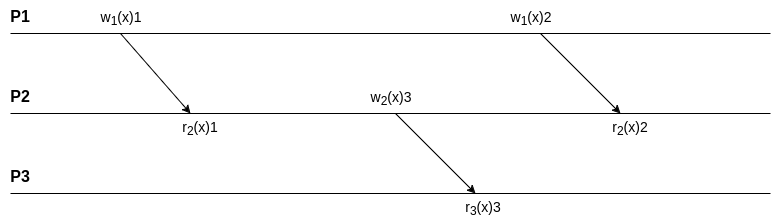
\includegraphics[width=\linewidth]{images/02-sequential.png}
    % [MB] a może "zachowujące spójność sekwencyjną"? gwarantować jej zachowanie może pewien schemat/algorytm, po czym następujące przetwarzania po prostu korzystając z gwarancji zachowują pewną własność. (moje językowe czepialstwo)
    \caption{Przetwarzanie zachowujące spójność sekwencyjną}
    \label{figure:replication_sequential}
\end{figure}

Obrazy historii w poszczególnych procesach wyglądają następująco:
\begin{align*}
    hv_1&: w_1(x)1 \rightarrow w_2(x)3 \rightarrow w_1(x)2 \\
    hv_2&: w_1(x)1 \rightarrow r_2(x)1 \rightarrow w_2(x)3 \rightarrow w_1(x)2 \rightarrow r_2(x)2 \\
    hv_3&: w_1(x)1 \rightarrow w_2(x)3 \rightarrow r_3(x)3 \rightarrow w_1(x)2
\end{align*}

Zwróćmy uwagę na fakt, że kolejność wykonywania zapisów jest każdym procesie taka sama, tj.\ $ w_1(x)1 \rightarrow w_2(x)3 \rightarrow w_1(x)2 $, a także, że kolejność ta jest zdeterminowana przez legalność uszeregowania w procesie $ P_2 $, dokonującym dwóch odczytów. Zauważmy, że aby zachować legalność uszeregowania w tym procesie odczyt $ r_2(x)1 $ musi następować po zapisie $ w_1(x)1 $ oraz przed zapisem $ w_2(x)3 $. Z kolei odczyt $ r_2(x)2 $, występujący po zapisie $ w_2(x)3 $ musi występować po zapisie $ w_1(x)2 $. Można więc powiedzieć, że proces $ P_2 $ dokonuje globalnego uszeregowania operacji zapisów w tym przypadku.

\subsubsection{Model spójności przyczynowej}

Model ten wymaga zachowania porządku przyczynowego operacji, tak jak zdefiniowany został w sekcji \ref{section:causal_order}. Dokładne omówienie modelu przyczynowego można znaleźć także w publikacji \cite{ahamad:95}. Jeśli operacja $ o_2 $ zależy przyczynowo od operacji $ o_1 $, to każdy z procesów musi wykonać operację $ o_1 $ przed wykonaniem operacji $ o_2 $, co formalnie zapisujemy:
\begin{align*}
    \forall_{o_1, o_2 \in O_i \cup OW} (o_1 \rightarrow o_2 \Rightarrow o_1 \mapsto_i o_2)
\end{align*}

Inaczej mówiąc, każde dwie operacje zapisu będące potencjalnie powiązane przyczynowo muszą być widziane przez wszystkie procesy w takim samym porządku. Zapisy współbieżne z kolei mogą być przez różne procesy oglądane w różnej kolejności, nie jest więc wymagane globalne uszeregowanie operacji zapisu. Sytuację taką pokazuje rysunek \ref{figure:replication_causal}.

\begin{figure}[t!]
    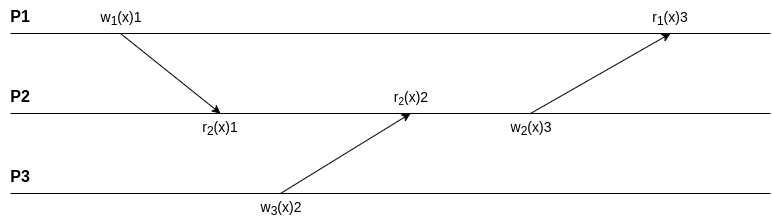
\includegraphics[width=\linewidth]{images/02-causal.png}
    % [MB] jw.
    \caption{Przetwarzanie zachowujące spójność przyczynową}
    \label{figure:replication_causal}
\end{figure}

Obrazy historii w poszczególnych procesach w przykładzie z rysunku \ref{figure:replication_causal} wyglądają następująco:
\begin{align*}
    hv_1&: w_1(x)1 \rightarrow w_3(x)2 \rightarrow w_2(x)3 \rightarrow r_1(x)3 \\
    hv_2&: w_1(x)1 \rightarrow r_2(x)1 \rightarrow w_3(x)2 \rightarrow r_2(x)2 \rightarrow w_2(x)3 \\
    hv_3&: w_3(x)2 \rightarrow w_1(x)1 \rightarrow w_2(x)3
\end{align*}

Zauważmy, że wśród zbioru operacji zapisu w systemie $ w_1(x)1 $ oraz $ w_3(x)2 $ są niezależne, natomiast operacja $ w_2(x)3 $ przyczynowo zależy zarówno od operacji $ w_1(x)1 $ jak i od $ w_3(x)2 $. Rzeczywiście, operacje $ w_1(x)1 $ oraz $ w_3(x)2 $ widziane są w obrazach historii w różnej kolejności, natomiast operacja $ w_2(x)3 $ zawsze występuje po obu wspominanych uprzednio operacjach.

\subsubsection{Model spójności PRAM}

Model spójności PRAM (\textit{ang.\ piplined RAM}) zapewnia zachowanie porządku zlecania operacji przez proces $ P_i \in P $ w obrazie historii każdego innego procesu. W sposób formalny powyższy warunek można zapisać następująco:
\begin{align*}
    \forall_{o_1, o_2 \in O_i \cup OW} ((\exists_{j=1..n} o_1 \rightarrow o_2) \Rightarrow o_1 \mapsto_i o_2)
\end{align*}

\begin{figure}
    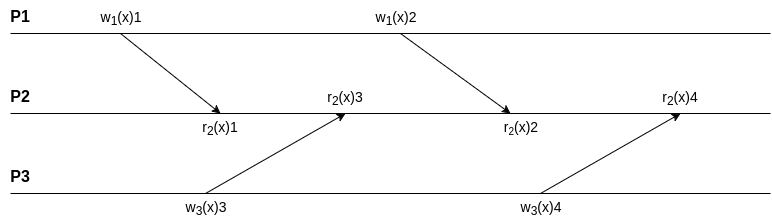
\includegraphics[width=\linewidth]{images/02-pram.png}
    % [MB] "zachowujące spójność PRAM"?
    \caption{Przetwarzanie zachowujące spójność PRAM}
    \label{figure:replication_pram}
\end{figure}

Obrazy historii w poszczególnych procesach w przykładzie z rysunku \ref{figure:replication_pram} wyglądają następująco:
\begin{align*}
    hv_1&: w_1(x)1 \rightarrow w_1(x)2 \\
    hv_2&: w_1(x)1 \rightarrow r_2(x)1 \rightarrow w_3(x)3 \rightarrow r_2(x)3 \rightarrow w_1(x)2 \rightarrow r_2(x)2 \rightarrow w_3(x)4 \rightarrow r_2(x)4 \\
    hv_3&: w_3(x)3 \rightarrow w_3(x)4
\end{align*}

Przykład przetwarzania w systemie zachowującym model PRAM został przedstawiony na rysunku \ref{figure:replication_pram}.

Należy zwrócić uwagę na to, że jedyne ograniczenia na lokalne obrazy historii jakie nakłada model
spójności PRAM to w tym przypadku konieczność, aby operacja $ w_1(x)1 $ poprzedzała $ w_1(x)2 $ oraz
aby operacja $ w_3(x)3 $ poprzedzała $ w_3(x)4 $, tzn.\ aby lokalne porządki wykonywania operacji w procesach $ P_1 $ i $ P_3 $ były zachowane w każdym procesie $ P_i \in P $. Więcej na temat tego modelu spójności można przeczytać w pozycji \cite{lipton:88}.

\subsubsection{Model spójności podręcznej}

Kolejny omawiany model spójności, tj.\ model spójności podręcznej, nazywany także modelem \textit{cache}, wymaga globalnego uporządkowania zapisów, ale tylko w odniesieniu do poszczególnych zmiennych. Innymi słowy, model ten nakłada ograniczenie, aby zapisy dotyczące zmiennej $ x \in X $ odbywały się w tej samej kolejności w całym systemie, jednak w przypadku zapisów do różnych zmiennych nie jest wymagane nawet zachowanie lokalnego uporządkowania operacji, model spójności podręcznej nie nakłada w takim przypadku żadnych ograniczeń. Formalnie powyższe stwierdzenie możemy zapisać w ten sposób:
\begin{align*}
    \forall_{x \in X} \forall_{w_1, w_2 \in OW \cap O|_x} (\forall_{i=1..n} w_1 \mapsto_i w_2 \vee \forall_{i=1..n} w_2 \mapsto_i w_1)
\end{align*}

Model spójności podręcznej jest całkowicie niezależny od modelu spójności przyczynowej oraz PRAM, możemy jednak zauważyć, że jest słabszy od modelu sekwencyjnego, ponieważ również wymusza jedną, globalną kolejność zapisów w systemie, przy czym robi to tylko w odniesieniu do poszczególnych zmiennych; nie mówi też nic o zachowaniu lokalnego uporządkowania operacji w każdym z procesów. Rysunek \ref{figure:replication_cache} przedstawia przykład przetwarzania zgodnego z modelem spójności podręcznej.

\begin{figure}
    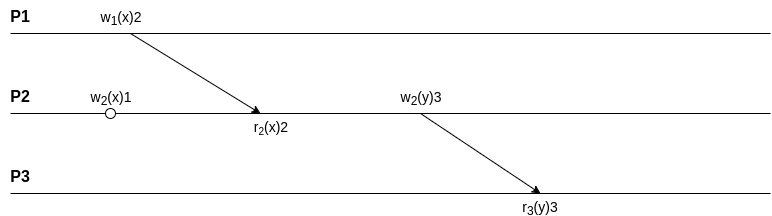
\includegraphics[width=\linewidth]{images/02-cache.png}
    \caption{Przetwarzanie gwarantujące zachowanie spójności podręcznej}
    \label{figure:replication_cache}
\end{figure}

Obrazy historii w poszczególnych procesach w przykładzie z rysunku \ref{figure:replication_cache} wyglądają następująco:
\begin{align*}
    hv_1&: w_2(x)1 \rightarrow w_1(x)2 \rightarrow w_2(y)3 \\
    hv_2&: w_2(x)1 \rightarrow w_1(x)2 \rightarrow r_2(x)2 \rightarrow w_2(y)3 \\
    hv_3&: w_2(y)3 \rightarrow w_2(x)1 \rightarrow w_1(x)2 \rightarrow r_3(y)3
\end{align*}

Zwróćmy uwagę, że jest to tylko jedno z wielu możliwych obrazów historii $ hv $, będących złożeniem lokalnych obrazów $ hv_i $ historii $ h $. Istotne jest to, że operacje zapisu do pojedynczej zmiennej (w tym przypadku do $ x $) są globalnie uszeregowane --- we wszystkich procesach zostają wykonane w tej samej kolejności. Jednocześnie, w procesie $ P_3 $ nie jest zachowywane lokalne uporządkowanie operacji z procesu $ P_2 $, ponieważ operacja zapisu $ w_2(y)3 $ w obrazie $ hv_3 $ historii występuje przed operacjami zapisu do zmiennej $ x $. Sytuacji takiej nie dopuści żaden z wcześniej opisywanych modeli, jednak w modelu spójności podręcznej taka sytuacja nie narusza ograniczeń.

\subsubsection{Model spójności procesorowej}

Warto wspomnieć także o istnieniu modelu spójności procesorowej. Nie wprowadza on nowych rodzajów ograniczeń, ale stanowi połączenie warunków zawartych w modelach spójności PRAM oraz podręcznej. Tak więc aby przetwarzanie było zgodne z tym modelem, lokalne obrazy $ hv$ historii $ h $ muszą zachowywać jednocześnie ograniczenia wprowadzone przez oba modele. Formalny zapis prezentuje się następująco:
\begin{align*}
    \forall_{o_1, o_2 \in O_i \cup OW} &((\exists_{j=1..n} o_1 \rightarrow o_2) \Rightarrow o_1 \mapsto_i o_2) \\
    \forall_{x \in X} \forall_{w_1, w_2 \in OW \cap O|_x} &(\forall_{i=1..n} w_1 \mapsto_i w_2 \vee \forall_{i=1..n} w_2 \mapsto_i w_1)
\end{align*}

Pracą poświęconą w dużej części tematyce spójności procesorowej jest m.in.\ \cite{ahamad:93}. Oczywiście zachowując model spójności procesorowej, gwarantujemy jednocześnie zachowanie zarówno modelu PRAM, jak i modeku spójności podręcznej. Przykładowe przetwarzanie w systemie zachowującym spójność procesorową zostało zobrazowane na rysunku \ref{figure:replication_cpu}.

\begin{figure}
    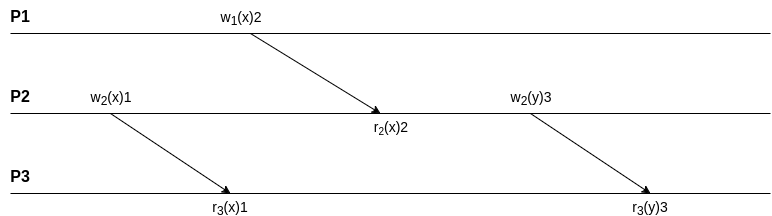
\includegraphics[width=\linewidth]{images/02-cpu.png}
    \caption{Przetwarzanie gwarantujące zachowanie spójności procesorowej}
    \label{figure:replication_cpu}
\end{figure}

Obrazy historii w poszczególnych procesach w przykładzie z rysunku \ref{figure:replication_cpu} wyglądają następująco:
\begin{align*}
    hv_1&: w_2(x)1 \rightarrow w_1(x)2 \rightarrow w_2(y)3 \\
    hv_2&: w_2(x)1 \rightarrow w_1(x)2 \rightarrow r_2(x)2 \rightarrow w_2(y)3 \\
    hv_3&: w_2(x)1 \rightarrow r_3(x)1 \rightarrow w_1(x)2 \rightarrow w_2(y)3 \rightarrow r_3(y)3
\end{align*}

Zauważmy, że zarówno lokalny porządek wykonywania operacji w każdym z procesów jest zachowany w każdym innym procesie (jest więc zachowany model spójności PRAM), jak i zapisy do tej samej zmiennej (w tym przypadku do $ x $) są globalnie uporządkowane --- mamy więc zachowany model spójności podręcznej. Ze złożenia obu warunków otrzymujemy, że przy założeniu powyższych lokalnych obrazów $ hv $ historii $ h $ w systemie zachowany jest model spójności procesorowej.

\subsubsection{Relacje pomiędzy danocentrycznymi modelami spójności}

Jak można łatwo zauważyć, przedstawione powyżej modele spójności nie są od siebie niezależne.
Opisywany w poprzednim punkcie model procesorowy jest złożeniem modeli: PRAM i spójności podręcznej,
jest więc od obu silniejszy. Nie jest to jednak jedyna zależność pomiędzy przedstawionymi modelami.
Można wykazać, choć dowody te nie mieszczą się w zakresie niniejszej pracy, że najsilniejszym z
przedstawionych modeli jest model sekwencyjny, tj.\ system gwarantujący zachowanie tego modelu w trakcie przetwarzania danych, gwarantuje jednocześnie zachowanie wszystkich innych modeli spójności. Model przyczynowy oraz procesorowy są od siebie niezależne, model PRAM jest słabszy zarówno od modelu przyczynowego, jak i procesorowego natomiast model spójności podręcznej jest słabszy od modelu sekwencyjnego i procesorowego oraz niezależny od pozostałych modeli. Sytuację tę obrazuje rysunek \ref{figure:replication_relations}.

\begin{figure}[H]
    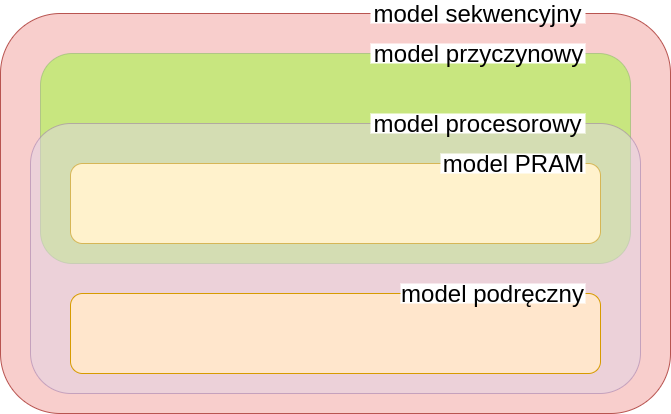
\includegraphics[scale=0.45]{images/02-relations.png}
    \centering
    \caption{Relacje zachodzące pomiędzy różnymi modelami spójności}
    \label{figure:replication_relations}
\end{figure}

Na powyższym rysunku zawieranie się prostokąta w innym oznacza, że odpowiadający mu model spójności jest słabszy od modelu oznaczonego prostokątem, w którym ten się zawiera.

\subsection{Modele klientocentryczne} \label{subsection:clientcentric}

Grupa modeli spójności klientocentrycznych, zwanych niekiedy gwarancjami sesji, obejmuje modele zapewniające pewne gwarancje klientowi odpytującego serwery o pewne dane, podczas jego interakcji z systemem (sesji). Zauważmy, że w przypadku poprednio omawianych modeli danocentrycznych nie było rozróżnienia na klientów i serwery, zakładały one, że procesy odwołujące się do rozproszonych danych są związane na stałe z jednym serwerem i nie przemieszczają się w czasie przetwarzania. Często jednak chcemy dopuścić możliwość separacji procesu aplikacyjnego od podsystemu zarządzania pamięcią, wówczas kolejne żądania do systemu mogą trafiać do innych serwerów ze względu na przemieszczanie się klienta, wykonującego te żądania. W takim przypadku potrzebujemy gwarancji innego rodzaju, a mianowicie takich, które respektują, że kolejne żądania jednego klienta do (potencjalnie) różnych serwerów nie są od siebie całkowicie niezależne. Dokładnie taka idea stoi za omawianymi w tym podrozdziale modelami klientocentrycznymi. Podane w bieżącej sekcji informacje nt.\ modeli spójności nastawionych na dane oraz sposoby ich uzyskania w środowisku rozproszonym dostępne są także w publikacji \cite{TDP+94}.

Dla lepszego zilustrowania znaczenia gwarancji wprowadzanych przez kolejne modele klientocentryczne, zamieszczony został poniżej rysunek \ref{figure:replication_sess_gu}. Następne podrozdziały będą odwoływały się do tego właśnie rysunku w kontekście prezentowanych przez nie klientocentrycznych modeli spójności.

\begin{figure}[H]
    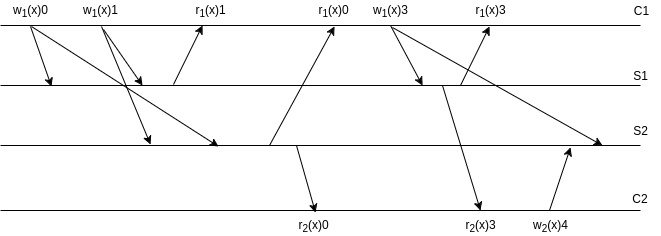
\includegraphics[width=\linewidth]{images/02-sess_gu.png}
    \caption{Przykładowe przetwarzanie w systemie z dwoma serwerami i dwoma klientami}
    \label{figure:replication_sess_gu}
\end{figure}

\subsubsection{Przyjęte oznaczenia}

Zanim zostaną przedstawione poszczególne modele klientocentryczne, należy wymienić i ściśle opisać oznaczenia, które zostaną użyte do formalnego zapisu wprowadzanych przez nie gwarancji przetwarzania. Oznaczenia te są następujące:

\begin{itemize}
    \item $ r $ operacja odczytu
    \item $ r|_{S_j} $ operacja odczytu wykonana na serwerze $ S_j $
    \item $ w $ operacja zapisu
    \item $ w|_{S_j} $ operacja zapisu wykonana na serwerze $ S_j $
    \item $ \xrightarrow{C_j} $ porządek operacji zlecanych przez klienta $ C_j $
    \item $ \xrightarrow{S_j} $ porządek operacji wykonywanych przez serwer $ S_j $
\end{itemize}

Należy w tym miejscu wprowadzić także definicję tzw.\ \textbf{zapisów odnośnych} (ang.\ \textit{relevant writes}). Skrót $ RW(r) $ oznacza zbiór zapisów, których wykonanie miało bezpośredni wpływ na wynik operacji odczytu $ r $.

\subsubsection{Read Your Writes}

Gwarancja \textit{Read Your Writes}, czyli \textbf{odczyt własnych zapisów} oznacza, że klient spodziewa się obserwować w każdej zlecanej przez siebie operacji efekty swoich poprzednich zapisów, nawet jeśli w międzyczasie nastąpiło przełączenie go na inny serwer. W sposób formalny, używając przyjętych oznaczeń, powyższy warunek możemy zapisać następująco:

\begin{align*}
    \forall{C_i} \forall{S_j} (w \xrightarrow{C_i} r|_{S_j} \Rightarrow w \xrightarrow{S_j} r)
\end{align*}

Praktycznym przykładem systemu, w którym gwarancja ta jest oczekiwana może być rozproszony system plików. Użytkownik wprowadza pewne modyfikacje w plikach na jednym komputerze, po czym kontynuuje pracę na innym komputerze i spodziewa się zobaczyć swoje zmiany wprowadzone wcześniej.

Odnosząc się do rysunku \ref{figure:replication_sess_gu} możemy zauważyć, że kolejne odczyty klienta pierwszego ($ r_1(x)1 $, $ r_1(x)0 $ i $ r_1(x)3 $) widzą zawsze jego wcześniejsze zapisy ($ w_1(x)0 $, $ w_1(x)1 $ w przypadku dwóch pierwszych odczytów oraz dodatkowo $ w_1(x)3 $ w przypadku ostatniego odczytu).
Odczyty $ r_2(x)0 $ oraz $ r_2(x)3 $ klienta drugiego nie są poprzedzone żadnymi zapisami tego klienta. Gwarancja sesji \textit{Read Your Writes} jest zatem \textbf{spełniona} w przedstawionym przetwarzaniu.

\subsubsection{Monotonic Writes}

Gwarancja \textbf{monotonicznych zapisów} (ang.\ \textit{Monotonic Writes}) oznacza, że kolejne zapisy klienta będą aplikowane na wszystkich serwerach w tej samej kolejności, innymi słowy zapisy poszczególnych klientów są globalnie uporządkowane. Formalna definicja tego warunku wygląda następująco:

\begin{align*}
    \forall{C_i} \forall{S_j} (w_1 \xrightarrow{C_i} w_2|_{S_j} \Rightarrow w_1 \xrightarrow{S_j} w_2)
\end{align*}

Przykładem dla zastosowania gwarancji \textit{Monotonic Writes} może być obiekt rozproszonego licznika, posiadający metody \texttt{ustaw} i \texttt{dodaj}. Licznik taki posiada w każdej chwili swój stan, dlatego aby zapewnić, że po serii modyfikacji wykonanych na nim przez jednego klienta stan wszystkich jego replik będzie taki sam, należy globalnie uszeregować wykonywane na nim operacje. Jeśli na każdym serwerze aktualizacje będą aplikowane w tej samej kolejności, wówczas końcowy stan będzie spójny.

Przykładowe przetwarzanie z rysunku \ref{figure:replication_sess_gu} możemy przeanalizować także pod kątem występowania tej gwarancji sesji bądź nie. Widzimy, że zapisy $ w_1(x)0 $ i $ w_1(x)1 $ na serwerze $ S_2 $ zostały zaaplikowane w kolejności innej niż kolejność zlecenia ich przez klienta. Tak więc gwarancja \textit{Monotonic Writes} \textbf{nie jest spełniona} w tym przetwarzaniu.

\subsubsection{Monotonic Reads}

Następną omawianą gwarancją sesji jest \textbf{monotoniczność odczytów} (ang.\ \textit{Monotonic Reads}). Polega ona na tym, że klient podczas każdej kolejnej interakcji z systemem widzi jego stan co najmniej tak samo aktualny jak podczas poprzedniej interakcji. Oznacza to, że jeśli już odczytano jakąś wartość $ v $ z systemu, to podczas żadnej z kolejnych interakcji klienta z systemem nie będzie możliwe odczytanie wartości starszej od $ v $, jeśli ma być zachowana gwarancja \textit{Monotonic Reads}. Powyższe zdanie w sposób formalny zapisuje się następująco:

\begin{align*}
    \forall{C_i} \forall{S_j} (r_1 \xrightarrow{C_i} r_2|_{S_j} \Rightarrow \forall{w_k} \in RW(r_1) (w_k \xrightarrow{S_j} r_2))
\end{align*}

Przykładem zastosowania gwarancji \textit{Monotonic Reads} jest skrzynka mailowa użytkownika. Jeśli raz odczytamy pewne wiadomości, to przy następnym sprawdzeniu zawartości skrzynki mailowej chcemy widzieć wszystkie te wiadomości. Innymi słowy, użytkownik nie powinien tracić dostępu do informacji, z którą już się zapoznał.

Patrząc na rysunek \ref{figure:replication_sess_gu} widzimy, że w przypadku każdych dwóch odczytów
zleconych przez dowolnego klienta, odczyt późniejszy widzi wszystkie zapisy, które miały wpływ na na
wyniki odczytane przez wcześniejszy odczyt, np.\ $ r_1(x)0 $ widzi zapisy $ w_1(x)0 $ i $ w_1(x)1 $, mające wpływ na odczyt $ r_1(x)0 $. Podobnie jest z parami odczytów: $ r_1(x)0 $ i $ r_1(x)3 $ oraz $ r_2(x)0 $ i $ r_2(x)3 $. W przypadku tego konkretnego przetwarzania gwarancja sesji \textit{Monotonic Reads} jest więc \textbf{spełniona}.

\subsubsection{Writes Follow Reads}

Ostatnią z przedstawionych w niniejszej pracy gwarancji sesji są \textbf{zapisy po odczytach} (ang.\ \textit{Writes Follow Reads}). Jest zastosowanie oznacza, że użytkownik chce respektowania przez system przyczynowej zależości pomiędzy zapisami, które wykonuje a poprzednimi odczytami. Innymi słowy, jeśli odczytamy wartość $ v $ z jednego serwera w systemie, po czym na podstawie tej odczytanej wartości decydujemy się na wykonanie zapisu w systemie, to poprzez zastosowanie gwarancji \textit{Writes Follow Reads} zapewnimy, że wszystkie serwery najpierw wykonają zapisy mające wpływ na odczyt wartości $ v $, a dopiero następnie nasz kolejny zapis, będący następstwem odczytu wartości $ v $. Formalna definicja wygląda następująco:

\begin{align*}
    \forall{C_i} \forall{S_j} (r \xrightarrow{C_i} w|_{S_j} \Rightarrow \forall{w_k} \in RW(r) (w_k \xrightarrow{S_j} w))
\end{align*}

Jako przykład systemu, w którym znaczenie miałaby gwarancja sesji \textit{Writes Follow Reads} może posłużyć lista dyskusyjna, w której użytkownicy mogą pisać wiadomości oraz odpowiadać na nie. Jeśli użytkownik odczyta treść pewnej wiadomości a następnie napisze odpowiedź do niej, to ważne jest, aby odpowiedź na oryginalną wiadomość została zapisana na każdym z serwerów po zapisaniu oryginalnej wiadomości. Innymi słowy, oprócz odpowiedzi na oryginalny list musi być zawsze widoczna treść oryginalnej wiadomości.

Rysunek \ref{figure:replication_sess_gu} przedstawia przetwarzanie, w którym w kontekście omawianej gwarancji sesji ważną obserwacją jest, że zapis $ w_2(x)4 $, następujący po odczycie $ r_2(x)3 $ nie jest świadomy wszystkich zapisów, które miały wpływ na wartość odczytaną w $ r_2(x)3 $ --- nie widzi bowiem zapisu $ w_1(x)3 $, który jest aplikowany na serwer $ S_2 $ dopiero po zapisie $ w_2(x)4 $.
